\documentclass[twocolumn,10pt]{asme2ej}

\usepackage{graphicx}
\usepackage{epsfig}
\usepackage{epstopdf}
\title{Sign language synthesis from Natural Language Processing}


\author{Nijat Mursali
\affiliation{
Department of Artificial Intelligence and Robotics\\
Sapienza University of Rome\\
}}

\begin{document}

\maketitle    

%%%%%%%%%%%%%%%%%%%%%%%%%%%%%%%%%%%%%%%%%%%%%%%%%%%%%%%%%%%%%%%%%%%%%%
\begin{abstract}
{
{\bf Abstract}—Sign language is a visual language used by individuals with speech and hearing impairments in order to communicate in their daily conversations. It is entirely an optical communication language due to its native grammar, which differs fundamentally from that of spoken languages.
The fundamental purpose of this paper is to describe an algorithm which takes the spoken language from the user, recognize word(s) with an algorithm and convert words to sign language. As an output, we display the images with the sign language. The method acts for primitive sentences as well as for compound ones, with some limitations, however. Two translation examples are given which illustrates main transformations done on the linguistic level. It is complemented by samples of images generated by the synthesize of the system.
}
\end{abstract}

\section{Introduction}

There are more than 7000 known living languages in the world divided in 136 different language groups. Among these 136 language families, Sign language is one and this family contains 136 sign languages all over the world depending upon the region of the world. Sign language is used by hearing impaired people to convey their message \cite{tamer-saraclar-2020-cross}. 

Sign language is a nonverbal language used by the deaf and hard of hearing to communicate using hand shapes, facial expressions, gestures, and other areas of the body. Because sign languages lack a well-defined structure or grammar, they have no or very little acceptance outside of their limited community. Approximately 72 million of the world's nearly 7 billion inhabitants are deaf or hard of hearing. Out of such a large population, roughly 4.3 million utilize Sign language. The remaining roughly 67 million deaf and hard of hearing persons do not communicate using any sign language. As a result, over 90 percent of the deaf have extremely limited or no access to schooling and other information. 

\subsubsection{Motivation}
The various advantages of building a speech to sign language system includes:
\begin{enumerate}
  \item Speech to sign language which includes more than 1000 words and phases and 26 English alphabetical letters can be used in several public domains.
  \item Speech to sign language system can help to translate the speech to text and then into the sign language which enables inter-communication between normal and deaf people.
\end{enumerate}

\subsubsection{Problem Statement}
Sign language uses many gestures to make it look like a movement language composed of a series of hand and arm movements. For different countries, there are different sign languages and gestures. In addition, sign language also includes specific gestures for each letter. Based on these sign languages, they are composed of two groups, namely static gestures and dynamic gestures. Static gestures are used for the representation of letters and numbers, while dynamic gestures are used for specific concepts. The dynamic also includes words, sentences, etc. Static gestures include gestures, while the latter include movements of the hands, head, or both. Sign language is a visual language made up of three main parts, such as finger spelling, word-level sign language vocabulary, and non-manual functions. Fingerprint spelling is used to spell words letter by letter and convey information, while the latter is based on keywords. Despite much research in recent decades, designing sign language translators remains a challenge. Furthermore, even the same logo has a significantly different appearance for different signers and different points of view. This work focuses on the creation of a static sign language translator by converting first speech to text and then applying the Natural Language Processing into the sentence and finally displaying the images of the words in sign language. As an outcome of application, we show set of images  We created a desktop application that can be used like a library for any type of application. 
\subsubsection{Objectives}
The fundamental goal of the project is to contribute to the field of speech to text translation and sign language. In our project, we focus on static sign language gestures. The focus of this work is the use of speech to text library to recognize the sentences. We implemented the Natural Language Processing algorithm in order to tokenize the words in the sentence and then by applying the algorithm to display the images in sign language. Our main application runs in Tkinter using Python programming language as a desktop application.

In the following sections we will be discussing how we developed the application that is capable of getting the speech from the user and giving the images of the sign language as output. The rest of this paper is organized as follows. Section 2 describes the literature review where we simply explain what kind of work has been done by other researchers. Section 3 discusses the data collection and how we have gathered the data, Section 4 explores the tool specification where we explain what kind of tools have been used for this project. Section 5 explores the implementation phase where we explain how we have developed the interface and algorithm. Then, Section 6 presents the results we have got for our algorithm. Finally, in Section 7 we conclude what have been done during this project and what can be done as future work.


\section{Literature Review}

This survey describes existing and established theories and research on sign language in American Sign Language. There are several types of ASL gestures that are used to recognize communication and we have different algorithms to recognize them. Communication plays a vital role in the interaction between people, it allows them to express themselves. Different methods are used to recognize American gestures that use different sign languages.
There is a huge gap in communication between normal and disabled people. Therefore, sign language can help communicate with disabled people. Different types of gestures are used and there are many forms in sign language. Similarly, the sign languages in different regions are also different and, to date, about 138 sign languages have been recognized \cite{1241384}. Anglo-American Sign Language is based on English, while Chinese and Indian sign languages have also been developed. Gesture-based sign language grammar ranges from written and spoken grammar, because gesture-based languages are based on forms and ideas, while, on the other hand, spoken and written languages include words and grammar rules. For this particular reason, the two languages have different grammatical structure \cite{servingdeaf}. The field of information technology has been strongly affecting human life. Different technologies, tools, and equipment have been developed to help humans solve various problems. Humans try to use information technology to bridge the communication gap between deaf and normal people. The concept behind this information technology-based tool helps deaf people to better communicate with people without disabilities and vice versa. This IT-based tool can be demonstrated in various situations \cite{american-interperete}. 

All modern technologies are related to mobile computing, gesture-based environments, and cloud computing. The world is entering the mechanism of gestures. IT companies like Microsoft, Google, and Leap Motion are releasing devices like the Kinect, Google Glass, and Leap Motion controllers, so the development of this technology can be used to benefit the deaf. For deaf children, communication is a huge waste \cite{Zafrulla2010AmericanSL}. They cannot integrate into society because they cannot communicate normally. In academia, the learning environment of deaf-mute students is not always parallel to that of normal students. One of the most effective ways for deaf people is to communicate through sign language. Experts or other personnel cannot understand communication through signatures through gesture-based interfaces. It creates difficulties in communication between deaf and normal people.

Sign language (SL) is the basic medium among people with hearing disabilities. This method is also called a dialect of optical movement. People who do not understand well use this method of sign language as the main channel of communication. Each country has its own sign language. For example, China, the United States, India, and Pakistan have their own sign languages, which are called Chinese Sign Language, American Sign Language, Indian Sign Language, and Pakistani Sign Language \cite{li2020wordlevel}. Many advanced countries made speeches on this topic. They organize different project activities, including information technology, to bridge the gap between deaf and normal people. Much research has been done on this topic in Central and South Asia. But so far, the main purpose of this research is to discuss issues between normal and deaf communities and after using the literature. They suggested many projects to build a bridge.

A good sign language recognition (SLR) system can break down the barriers between language and listening communities and language culture. The goal of SLR is to create methods and methods that correctly recognize a series of gestures and understand the meaning of the gestures. SL raises a question because it is multi-channel and interprets meaning in multiple ways at the same time. Due to some limitations and variables, SLR is a challenging and motivating task \cite{DBLP}. This is not an easy task, because we cannot always use precise stages to convert to ASL. Therefore, we must find a way to process the dataset and complete the task.

To recognize sign language, Lionel et al. Performed this process in two steps. They are extraction of characteristics and classification of actions. This process is also carried out using neural networks and using Microsoft kinnect. Lionel collected 20 different Italian gestures, which were signed by 27 people around. Using Microsoft kinnect to record the video, he used a total of 6,600 images, of which 4,000 images were submitted for training, with the remaining images submitted for testing or verification. For model learning, only one side is used and the maximum combination is used to extract features. The model contains two outputs, which are combined and delivered to the ANN. To extend the data, the CPU is used and the GPU is used to train the model. The downside of this process is that the output accuracy of the training model is low, close to 72.5\% \cite{signrecog}.

(Greive Smith, 1999) \cite{englishtoamerican} Use weather forecast information as a natural language sentence, label each word according to the meaning of each word, and use the domain-defined top-down recursive parser to parse the sentence to complete a pre-formatted Table. Then, the system applies each word to the translation rules and reconstructs the sentence. However, this method is only suitable for specific fields where the number of words used is limited and the sentence structure is standardized.

To overcome the above problems, we analyze the data not at the word level but at the sentence level, and apply rules that take advantage of the difference between American and Sign Language. 

\section{Data collection}

We have created a new dataset of ours by gathering the sign language images from different sources. The fundamental approach was to use some phases which gave us the opportunity to get images of sign language for different words. Since parsing all the images manually would not be a good idea, thus we have created a new function in order to call the links automatically and parse the images from all of those links. We have used {\emph BeautifulSoup} for this and for all the letters in English language (A-Z) we have checked every single link for the images and added them to local storage. 

To explain in details, to gather the data we have used BS4 where we first add all the alphabetical letters in English language (A to Z) to the list. The good side of using BS4 is that it can iteratively check the link for all the letters for our list. We managed to achieve this by \verb|?letter={letter}| which checks all the letters we have in our list. Normally, for first argument in BS4, you need to have response where we could get by using \verb|requests.get(url)| for each of the letters. After getting the response, we add it to BS4 as argument, then we check the content by \verb|soup.find_all()| function. If we have the specific element we are looking for, we add them to the new list for anchor tags. Next, we check for all the links the specific tag where the images are initialized. If image is found, then we use the PIL library to open, resize and save the images to the local storage. 

\begin{figure}[h]
    \centering
    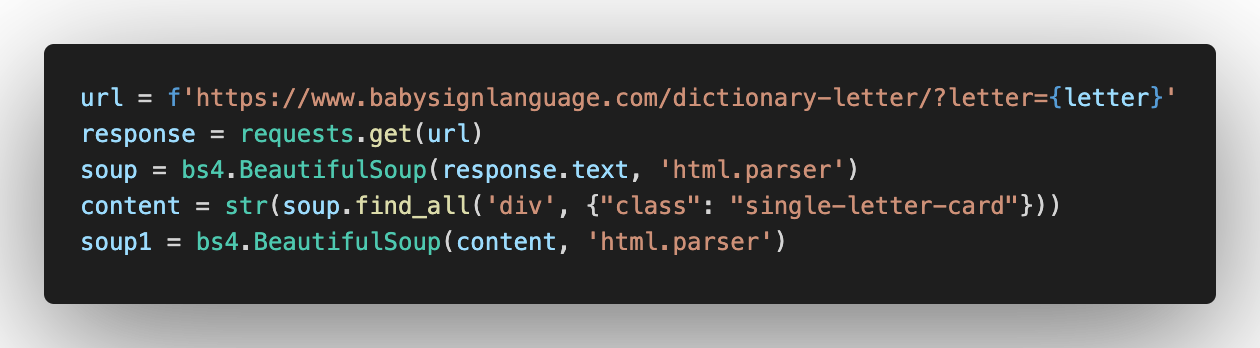
\includegraphics[width=0.5\textwidth]{figure/fig1.png}
    \caption{Getting the links for all letters}
    \label{fig:mesh1}
\end{figure}
As shown in the image, we have first added all the alphabet letters in English language and for those letters, we have checked the URL response and for specific element we get all the links. Then we have added those links to the list for further processing. 

Then, for all the links, we are making the GET request for specific elements where images are added by their source and name. Then, within the loop, we are making the request to get the images and add them to the local storage. 

\section{Architectural Framework}
This research presents an architectural framework of American sign language recognition tool developed to convert speech to sign language. By using this particular tool, the speech can be converted the speech into text by using Google TTS. An architecture of this recognition has been presented in Figure 2. The system accepts the input in the form of a speech from microphone of the user and translates the speech to text and then to sign language. 

\begin{figure}[h]
    \centering
    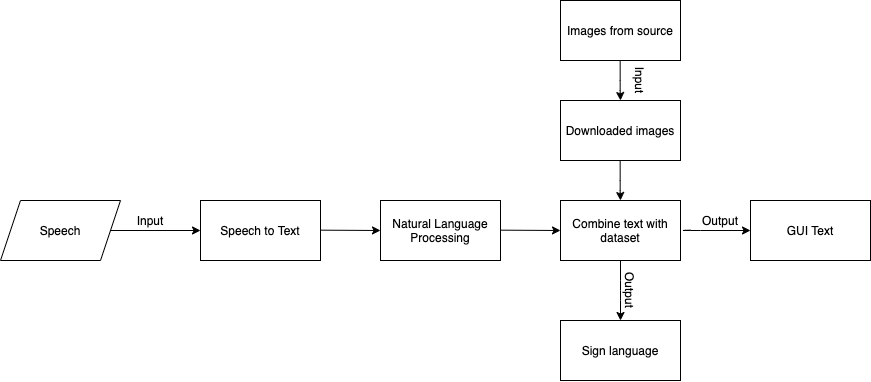
\includegraphics[width=0.5\textwidth]{figure/Untitled Diagram.png}
    \caption{Getting the links for all letters}
    \label{fig:mesh1}
\end{figure}

\subsection{Tool specifications}
In this section we will explain which tools we have used to develop the whole application by including the information about the programming language, GUI, natural language processing and displaying the imaged as output.  
As a fundamental programming language, we have used Python. Python is an interpreted high-level general-purpose programming language. Python's design philosophy emphasizes code readability with its notable use of significant indentation. 
For the GUI, we could use several Python libraries, but the best library for GUI in Python is Tkinter. Tkinter is a Python binding to the Tk GUI toolkit. It is the standard Python interface to the Tk GUI toolkit, and is Python's de facto standard GUI. Tkinter is included with standard Linux, Microsoft Windows and Mac OS X installs of Python.

In order to get all the images we have used Beautiful Soup. Beautiful Soup is a Python package for parsing HTML and XML documents. It creates a parse tree for parsed pages that can be used to extract data from HTML, which is useful for web scraping. 

After having all the image sources, we had to find a way to download all images automatically. For this purpose, we have used PIL library which stands for Python Imaging Library that is a free and open-source additional library for the Python programming language that adds support for opening, manipulating, and saving many different image file formats. For this case, we have got the names of the images from the source and split the name. Then, we have opened the image with PIL library and resized all of them to be 512x512 format and then saved all the images. 

\subsection{Speech and NLP}
In order to get the speech from the user, we have used speech recongition library in Python. The fundamental idea here is to initialize the microphone by calling the library and then get the audio from the microphone. In order to recognize the audio, we have used \textit{SpeechRecognition} library. We first initialize the Recognizer class is used to recognize the speech. Each Recognizer instance has seven methods for recognizing speech from an audio source using various APIs. We have used \textit{recognize google}. Finally, we use the microphone as a source and get the audio by sendin the \textit{listen} for the source. As a result of this process, we get the sentence as text variable. 

For this part, we have used Python's NLTK library. NLTK stands for The Natural Language Toolkit, or more commonly NLTK, is a suite of libraries and programs for symbolic and statistical natural language processing for English written in the Python programming language. 

In order to display the images, we have added all the images as output to the list. Then, we have saved all the images inside the GIF file. Next, by using the webbrowser library we have opened the output file in the new browser. 

We have used the {\emph Tkinker} which is a Python binding to the Tk GUI toolkit. It is the standard Python interface to the Tk GUI toolkit. We have created a simple interface where the user can click the button to get the speech from the user and then the algorithm will check which words the user has said. The following image shows the interface of the application.

\begin{figure}[h]
    \centering
    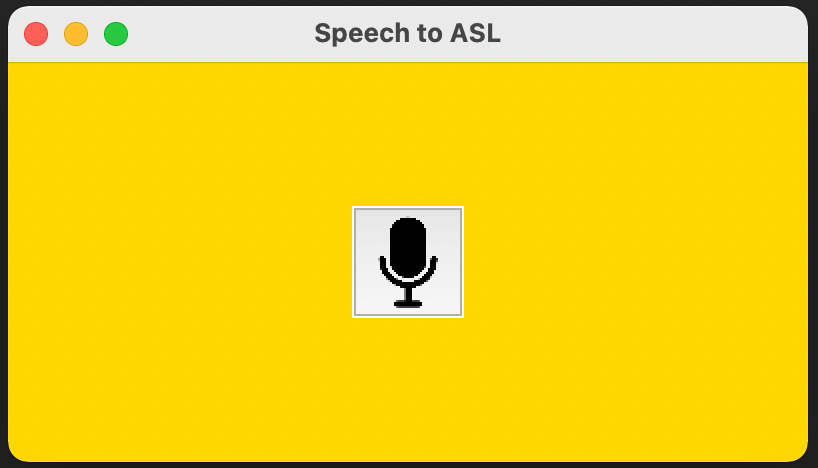
\includegraphics[width=0.4\textwidth]{figure/fig2.png}
    \caption{Getting the links for all letters}
    \label{fig:mesh1}
\end{figure}

In order to get the input from the microphone, you need to press the microphone button. After pressing the button, the input is recorded and added to a variable called "text". 

\section{Algorithm}

We started with the set of 1000 images for our dataset by applying our code from scratch. The fundamental idea was to add all the alphabetical letters in English (A-Z) and checking the URL for all those letters in a loop. For each of those letters, we loop through all the links for those letters and check if we have the specific anchor tag element for that response. In our case, we have checked the \textit{div} element if it has the special class. If yes, we added the \textit{href} (an attribute of the anchor tag) elements to the list. For the next step, in a loop for each element of that list, we have checked if the link contains the image tag. If yes, we have used PIL library to resize and save the images to local system. 

The fundamental step for the algorithm part was the base of the code where we first got the sentences from the user. As we explained, we used microphone in order to get the input from user and by using the Google Speech API we managed to add the speech to text variable. As we store the text variable (which is a string), we then moved to NLTK where we divided the sentence into words by tokenizing them. 

In the following process, we used NLTK Python library to convert the sentence into array of words and then tokenize those words by also checking if we have stopwords. We use {\emph "word tokenize"} from NLTK library to get the tokenized words. Tokenizing allowed us to easily break up text by word or phrase. Then it allowed us to deal with smaller chunks of text that are still pretty cohesive and intelligible even when taken out of context. It was the initial stage in transforming unstructured data into structured data that could be analyzed more easily. Normally, there are two ways to tokenize: word and sentence. In our case, we have used word tokenize because we needed to deal with stand alone words. 

For this process, we also check if sentences have some punctuations. As we know, in English language "{\emph '}" is used quite often. When we use NLTK library, this could cause misdivisions of the sentence. Thus, we just removed the punctuations. Another fundamental step was to check the stopwords. Stop words are words that you wish to ignore, so while you're processing text, you filter them out. Because they don't contribute much sense to a sentence, common words like 'in,' 'is,' and 'an' are frequently employed as stop words. We have then added a new empty list and by checking the stop words in the sentence we add the important words to our list in order to display the set of images in sign language as an output. 

Another step for NLP part was to use stemming for our algoritm. Stemming is a text processing task in which you reduce words to their root, which is the most important element of the term. For example, the roots of the words "helping" and "helper" are the same. Stemming helps you to focus on the fundamental meaning of a word rather than the specifics of how it is used. There are other stemmers in NLTK, but you will be utilizing the Porter stemmer. After checking the stopwords, we have used Porter's stemmer in order to bring the words to their initial roots. For instance, if we say "I am going to buy flowers." if we use stemmer, the output will be "['i', 'am', 'go', 'to', 'buy', 'flower']" which brings all the words to their initial forms. 

The next step for our algorithm was to check the words and images for those words in our database. As we have mentioned earlier, we collected to add more than 1000 words for our dataset. We know that it is not always possible to have all the words in the dataset, so for that case we are using the alphabetical characters in English language. So, basically, if a NLP tokenized sentence contains the word that is in our dataset we add that image to the list, otherwise we divide the word into characters of letters and adding image in sign language for each of those letters. 

As a final step, we have used the {\emph webbrowser} library which comes with Python to export the images to GIF file in order to display them in the new browser. For the images, we previously added all the images to the list which contains the path of all of the images in the system. Thus, by using the library, we append the images and save the images to GIF file and open the GIF in new tab by using the webbrowser. 

\section{Results}
{\bf Steps 1:} A window appears on the screen and it
allows the user to choose any one of the languages among
the available languages in the following figure. Fig.2.

{\bf Steps 2:} After pressing the microphone button, user is asked to talk to microphone. Whenever, user finishes talking, the algorithm starts to check the sentence by using natural language processing tools. 

{\bf Steps 3:} After user speaks, the user can see the output text message of what he has spoken through the microphone. So, the speech recognition library recognizes the speech and adds to text string. These kinds of output pop-up windows shown in the figures are displayed only when we use the Tkinter package in the code. By using Tkinter, we show that text in pop-up window. Fig.3.

\begin{figure}[h]
    \centering
    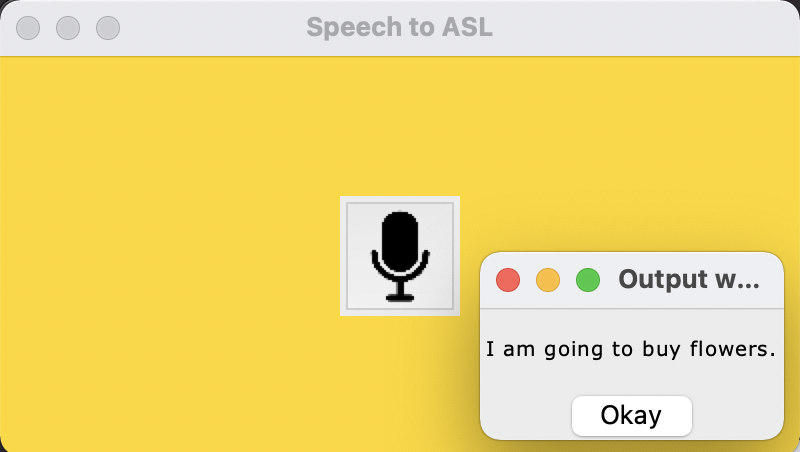
\includegraphics[width=0.4\textwidth]{figure/output_speech.png}
    \caption{Output of spoken language into ASL}
    \label{fig:mesh1}
\end{figure}

{\bf Steps 4:} Final step is to check the sentence user have spoken and. by the help of NLTK, we divide the sentence into words and tokenize the words by bringing them to their root. As we have the words, we have checked if those words are in our dataset or not. If we have the words in our dataset, we add the image to the array, if not we check the characters of that word and add the alphabetical letter to the image list. 

The actual test session was composed of a set of several tasks like simple sentences. We asked some users to try some simple sentences with our algorithm. We have received sentences from a total of 10 subjects (5 women and 5 men) were involved in the experiments. The subjects were all students, 22-25 years old. Each user was asked to perform to say 5-10 simple sentences. Most of the sentences were like "I am going to home", "I go supermarket", "I love parents" and etc. 

For each of the users, measures were acquired regarding the number of fully successfully tasks and the number of partial failures (attempts that needed to repeat the interaction at least once to get the task successfully completed). The measures are reported in Table I for one user. We have added 5 sentences to the table by showing the success and failure rates. 

\begin{table}[h!]
\begin{center}
\begin{tabular}{ |c|c|c|c| } 
\hline
{\bf Sentence} & {\bf Successful} & {\bf Partial Failure} \\
\hline
I want to buy flowers. & 100\% & 0\% \\ 
I like eating apple. & 100\% & 0\% \\ 
He is nice guy. & 70\% & 30\% \\ 
I like school. & 100\% & 0\% \\ 
He is tall student. & 80\% & 20\% \\ 
\hline
\end{tabular}
\end{center}
\caption{Table to test captions and labels}
\label{table:1}
\end{table}


As we have previously mentioned, to test the proposed work, we have taken some simple sentences from other users as well. For the moment, we take simple sentences with 2-5 words,thus we have taken mostly used English words and sentences into consideration. Given the low number of words in the sentence to the tests, the very high score in algorithm was easily expected. However, in real scenario, it does not always work, and we might sometimes have longer sentences. For instance, in above table, we have a failure for "He is nice guy" example, because our algorithm does not have "is" and "guy" in our dataset, thus it gets the alphabetical letters for those words. The same thing appeared with "he is tall student" example because we again did not have some words in our dataset. 

During our testing process, we have met several problems. One problem we have saw during our testing process was about low quality of audio input. Some laptop microphones don't provide high quality audio input or noise canceling. Because of this reason, sometimes the algorithm detects other sounds as well. Another problem we faced was with speech recognition. The users were from different countries, while the interaction with the algorithm was entirely in English. As a consequence, the small fraction of partial failures, also pointed out in the responses to the user experience questionnaires, might also be originated by an imperfect pronunciation.

In the next subsection we have showed some example we have checked in our testing session. We will first explain how we get the sentence, then explaining how the sentence is tokenized and finally showing the output image for the sentence.

\subsection{Experiments}
\subsubsection{Experiment 1}
As a first example, we can say the sentence is "I wanted to go to America." In this case, if we tokenize the words, we will get the list of words which are "I", "want", "to", "go", "america". Thus, our application checks every words in the dataset, if it exists or not, so if yes, it adds the image to the list of images. If the image does not exist in the dataset for that specific word, it divides the words into characters and adds the alphabetical character of each word into the list of images. For instance, in our sentence we had "to", so we can show it as an alphabetical characters. The following figure shows the output of the sentence we have mentioned above. 

\begin{figure}[h]
    \centering
    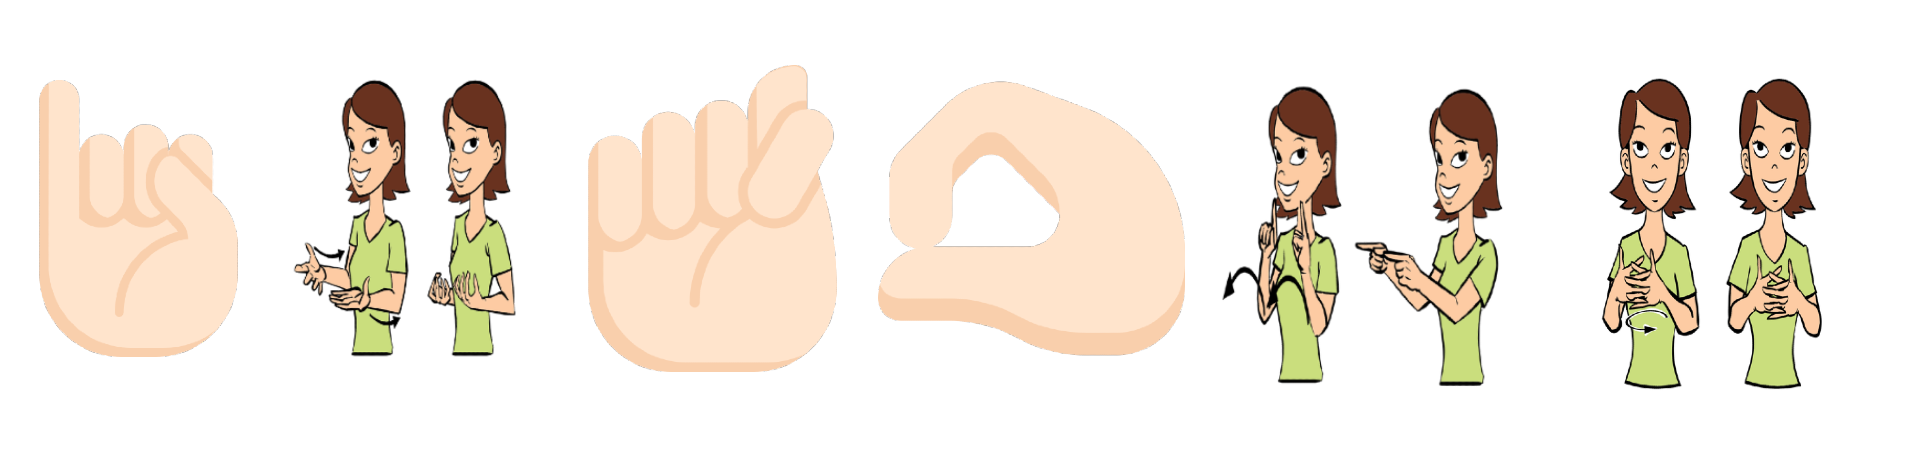
\includegraphics[width=0.4\textwidth]{figure/Untitled.png}
    \caption{Output of spoken language into ASL}
    \label{fig:mesh1}
\end{figure}

\subsubsection{Experiment 2}

For another example, we have chosen the sentence "Today I will plant trees in garden". As seen from the sentence, we have different type of words in the sentence. If we check it, we have three stop words in this case: I, will and in. For our algorithm, we actually don't need to have will and in and we don't need to convert them to sign language. Thus, by using the algorithm, we managed to remove the stopwords from the sentence. 


Words like "I" may seem too important to filter out, and depending on what kind of analysis you want to do, they can be. The fundamental reason for it is that "I" is a pronoun which is a context word instead of a content word. For this reason, we needed to have "I"in the sentence because it has it's own meaning. Thus, the final tokenized sentence without stopwords will be like "today I plan tree garden". Here we just needed to get the important words and display the output images for those words. The following figure shows the output of the sentence we have mentioned above. 

\begin{figure}[h]
    \centering
    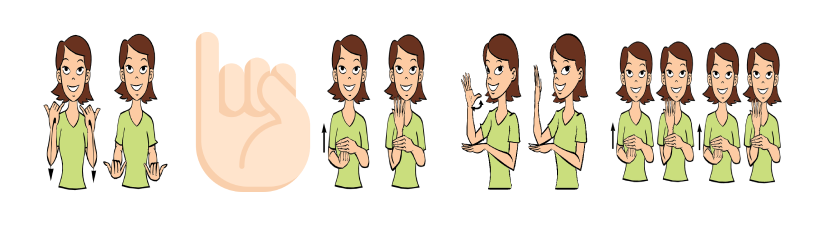
\includegraphics[width=0.4\textwidth]{figure/New Project.png}
    \caption{Output of spoken language into ASL}
    \label{fig:mesh1}
\end{figure}

\section{Conclusions and Future Work}
This research paper exhibits an optimal approach, to accomplish the algorithm which makes it possible to get the speech input from the user and apply the Natural Language Processing (NLP) to convert the words to initials forms and display the images of the words in sign language. In order to accomplish this task, we have gathered around more than 1000 images and 26 alphabet letters in English language. For the NLP, we have used specific NLTK library and algorithms to convert the words into the initial form. We also took the some specific punctuations in English language. Thus, if no word is in the database, it checks the characters of the unknown word and displays the images of letters in English alphabet.   
The functionalities of the proposed system can be expanded to identify more complex sentences by adding our dataset of images which could explain the phases in English language. 

\begin{acknowledgment}
I would like to thank my professor Christian Napoli for his guidance throughout this project. I would also give my huge thanks to my colleagues for testing the application and specifying the accuracyy the have got for this project. 
\end{acknowledgment}

\addcontentsline{toc}{chapter}{Bibliography}
\input{References}

\end{document}
